\section{Appendix: Handwritten records of the experiment}
\label{sec:records}
%    \includegraphics[width=\linewidth]{appendix/}
%\clearpage
\FloatBarrier

\section{Appendix: Plots for measurement of different gratings.}
\label{sec:appendix_gratings_plots}
\begin{figure}[H]
    \centering
    \begin{subfigure}[b]{\mpltw}
        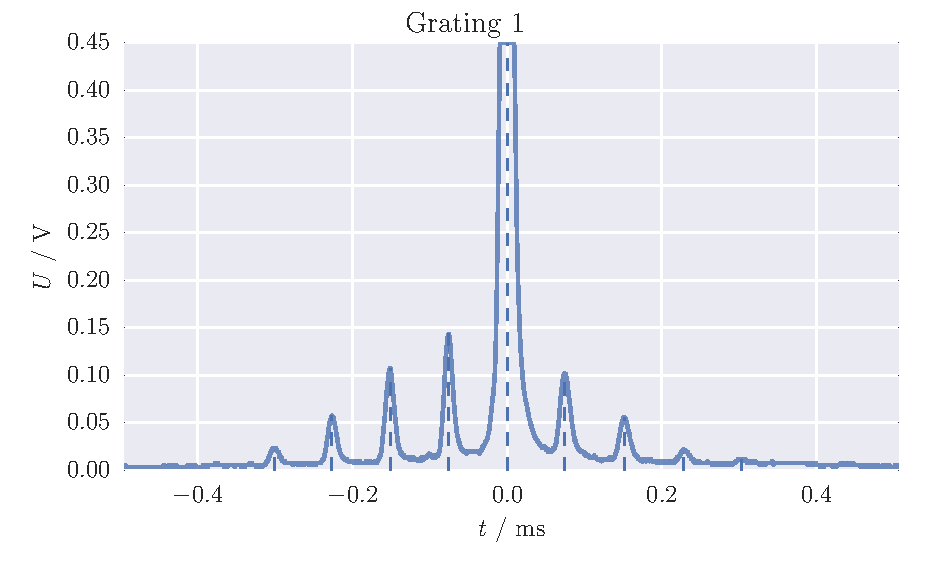
\includegraphics[width=\textwidth]{figures/gratings_maxi1}
        \caption{Grating 1}
        \label{fig:gratings_maxi1}
    \end{subfigure}\quad
    \begin{subfigure}[b]{\mpltw}
        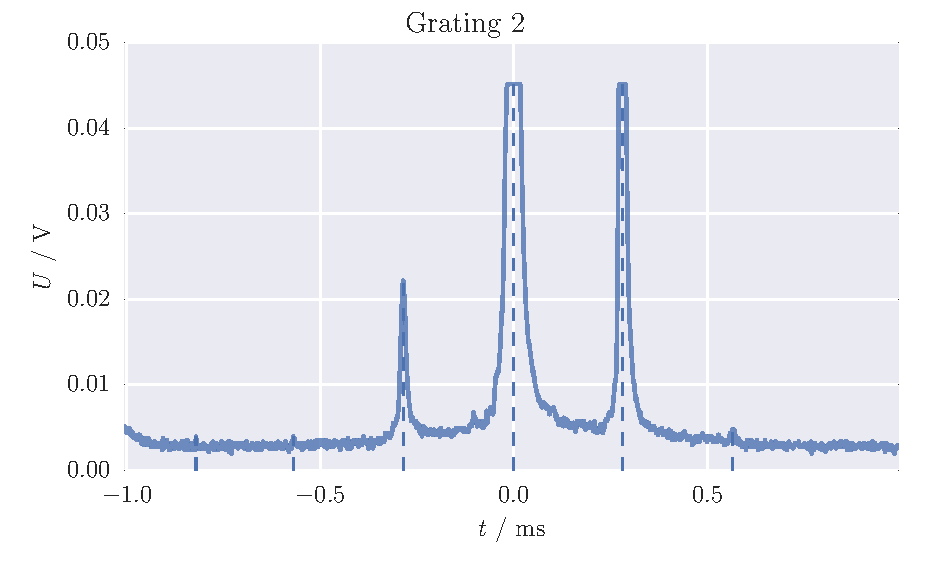
\includegraphics[width=\textwidth]{figures/gratings_maxi2}
        \caption{Grating 2}
        \label{fig:gratings_maxi1}
    \end{subfigure}
    \begin{subfigure}[b]{\mpltw}
        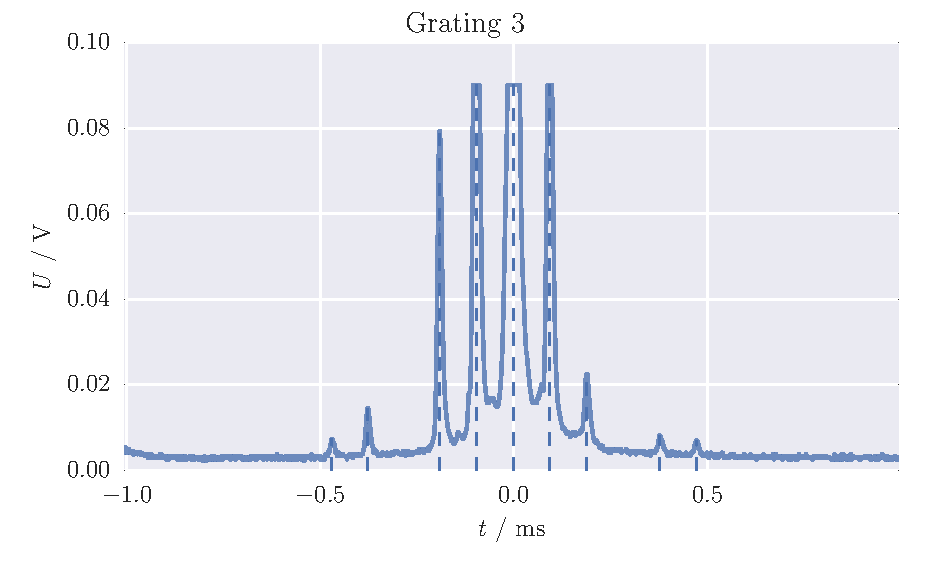
\includegraphics[width=\textwidth]{figures/gratings_maxi3}
        \caption{Grating 3}
        \label{fig:gratings_maxi1}
    \end{subfigure}\quad
    \begin{subfigure}[b]{\mpltw}
        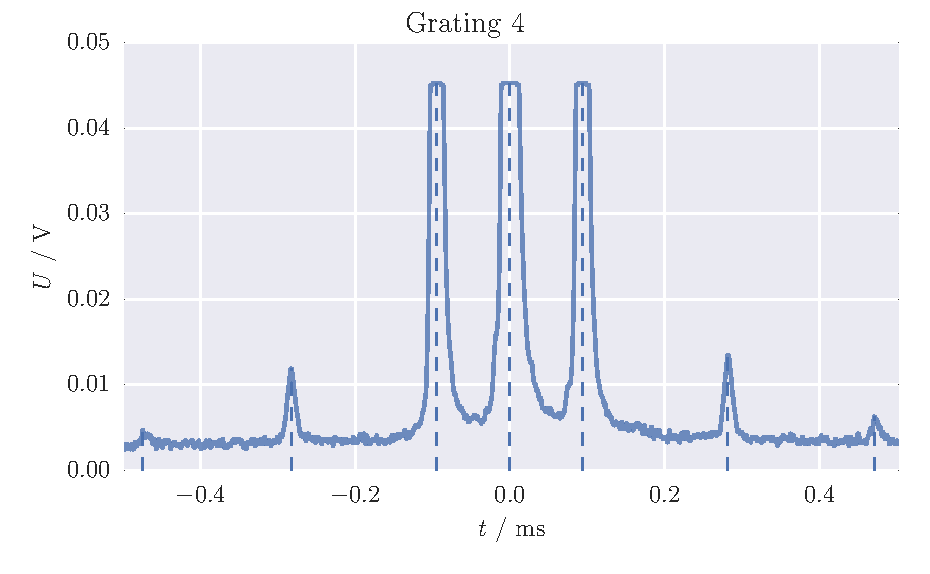
\includegraphics[width=\textwidth]{figures/gratings_maxi4}
        \caption{Grating 4}
        \label{fig:gratings_maxi1}
    \end{subfigure}
    \begin{subfigure}[b]{\mpltw}
        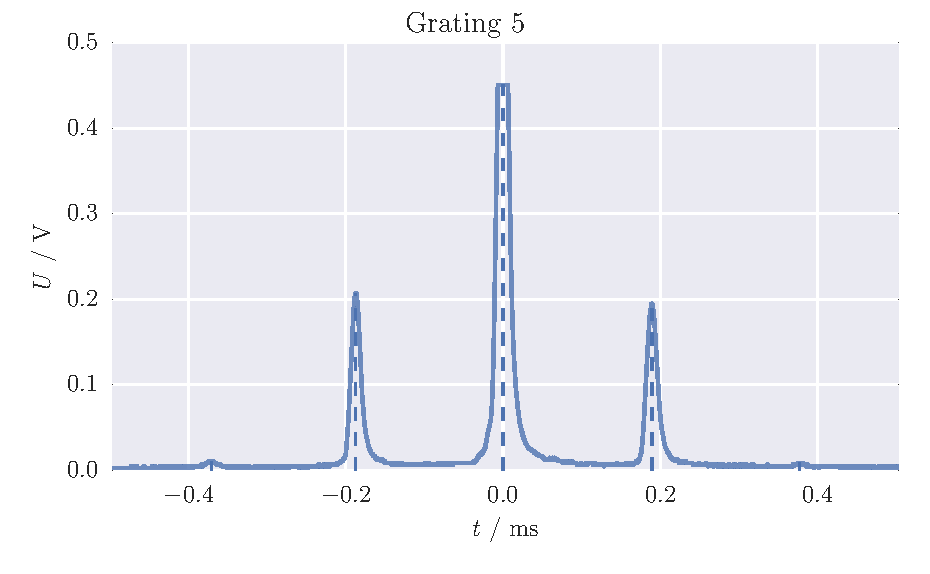
\includegraphics[width=\textwidth]{figures/gratings_maxi5}
        \caption{Grating 5}
        \label{fig:gratings_maxi1}
    \end{subfigure}
    \caption{
        Measured spectra of gratings with maxima numerically found (shown as broken 
            lines). The maximum of zeroth order is not used in the analysis. 
        }
    \label{fig:gratings_maxima}
\end{figure}
\FloatBarrier

\section{Appendix: Plots for measurement of different gratings.}
\label{sec:appendix_aperture_plots}
\begin{figure}[H]
    \centering
    \begin{subfigure}[b]{\mpltw}
        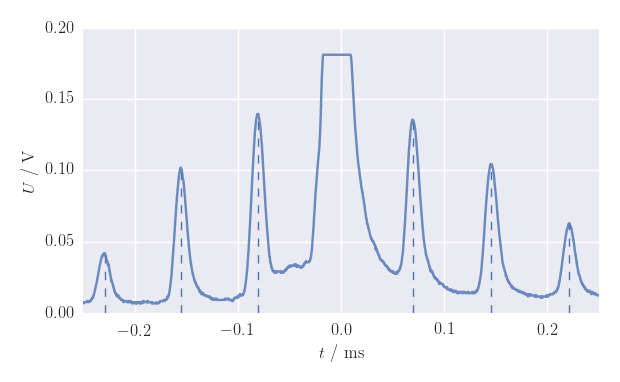
\includegraphics[width=\textwidth]{figures/aperture_1b}
        \caption{Position 1}
        \label{}
    \end{subfigure}
    \begin{subfigure}[b]{\mpltw}
        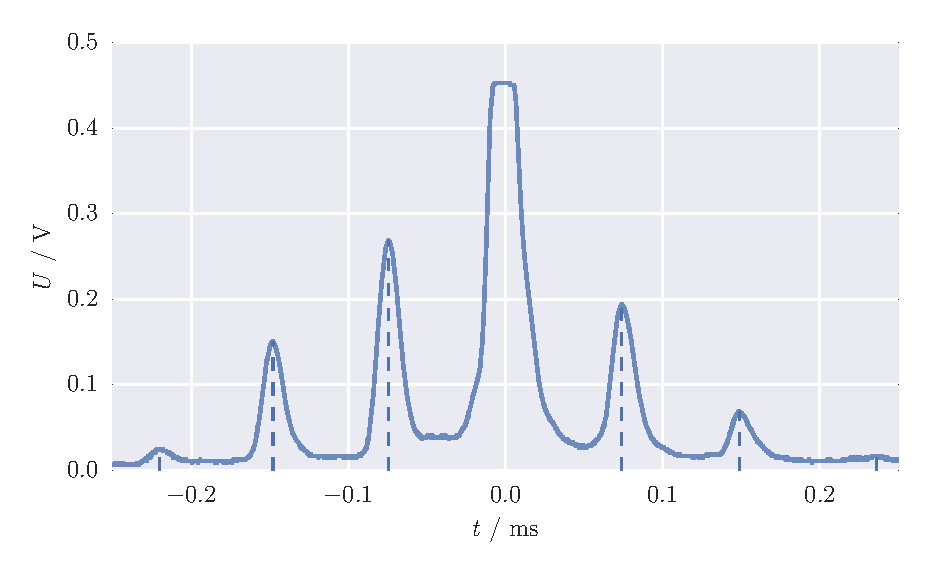
\includegraphics[width=\textwidth]{figures/aperture_2b}
        \caption{Position 2}
        \label{}
    \end{subfigure}
    \begin{subfigure}[b]{\mpltw}
        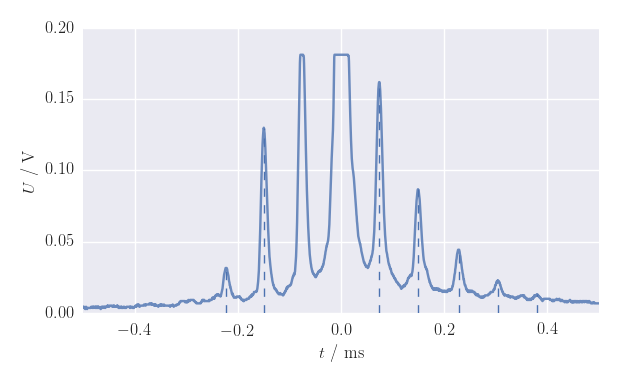
\includegraphics[width=\textwidth]{figures/aperture_4b}
        \caption{Position 4}
        \label{}
    \end{subfigure}
    \begin{subfigure}[b]{\mpltw}
        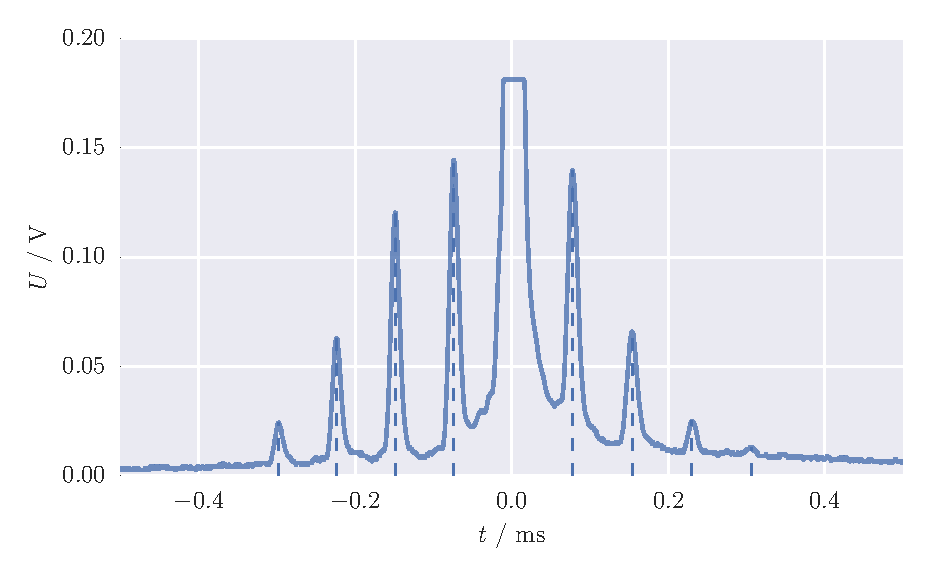
\includegraphics[width=\textwidth]{figures/aperture_5b}
        \caption{Position 5}
        \label{}
    \end{subfigure}
    \begin{subfigure}[b]{\mpltw}
        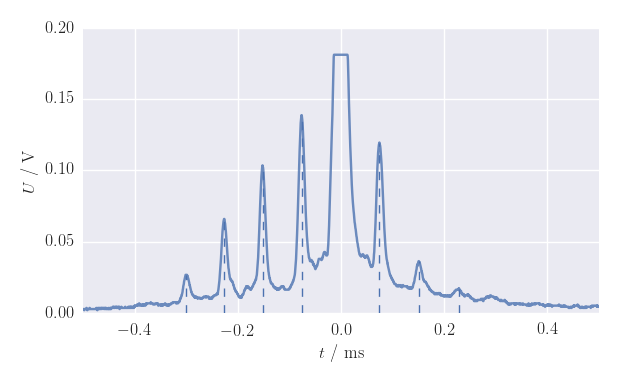
\includegraphics[width=\textwidth]{figures/aperture_6b}
        \caption{Position 6}
        \label{}
    \end{subfigure}
    \begin{subfigure}[b]{\mpltw}
        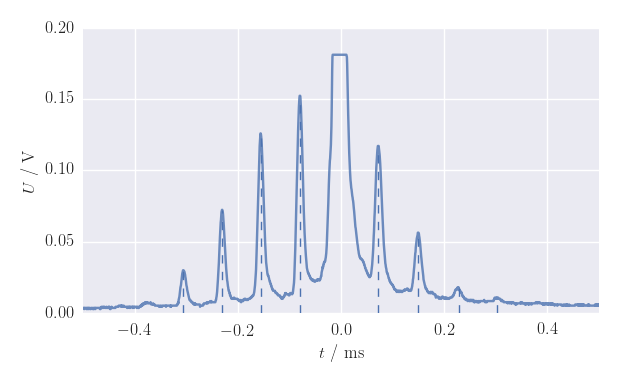
\includegraphics[width=\textwidth]{figures/aperture_7b}
        \caption{Position 7}
        \label{}
    \end{subfigure}
    \begin{subfigure}[b]{\mpltw}
        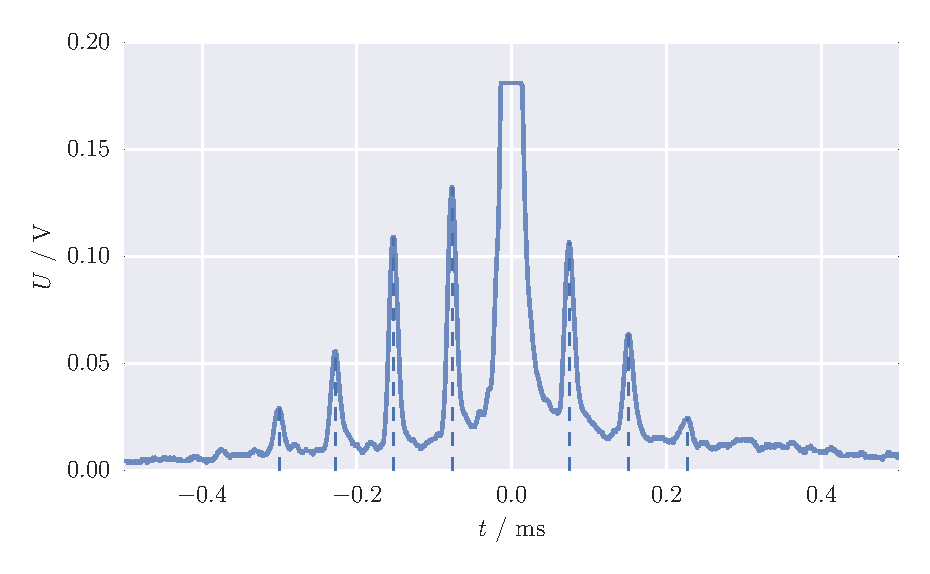
\includegraphics[width=\textwidth]{figures/aperture_8b}
        \caption{Position 8}
        \label{}
    \end{subfigure}
    \caption{
        Measured intensities for grating one for different positioning of the grating.
        In order to get the magnitude of the zeroth order maximum, we took other measurements 
        on a larger scale. Only the first plot shows decent symmetry, but only 
        maxima to the 3rd order are observed. We decided to use the measurement 
        at position 5 for the approximation of the aperture function, showing maxima 
        up to the 4th order. 
        }
    \label{fig:aperture_positions_detail}
\end{figure}

